\section{40GBASE-T}

\subsection{Wprowadzenie}
40GBASE-T jest technologią transmitowania ramek Ethernetowych z prędkością 40 gigabitów na sekundę, wykorzystując skrętkę jako medium. Technologia została zdefiniowana po raz pierwszy jako część standardu IEEE 802.3ba w 2010 roku.

40GBASE-T zapewnia dwukierunkową komunikację przez cztery przewody skrętki. Każdy przewód transmituje ¼ zgromadzonych danych.

\subsection{Położenie 40GBASE-T w modelu OSI}

\begin{figure}[ht]
    \centering
    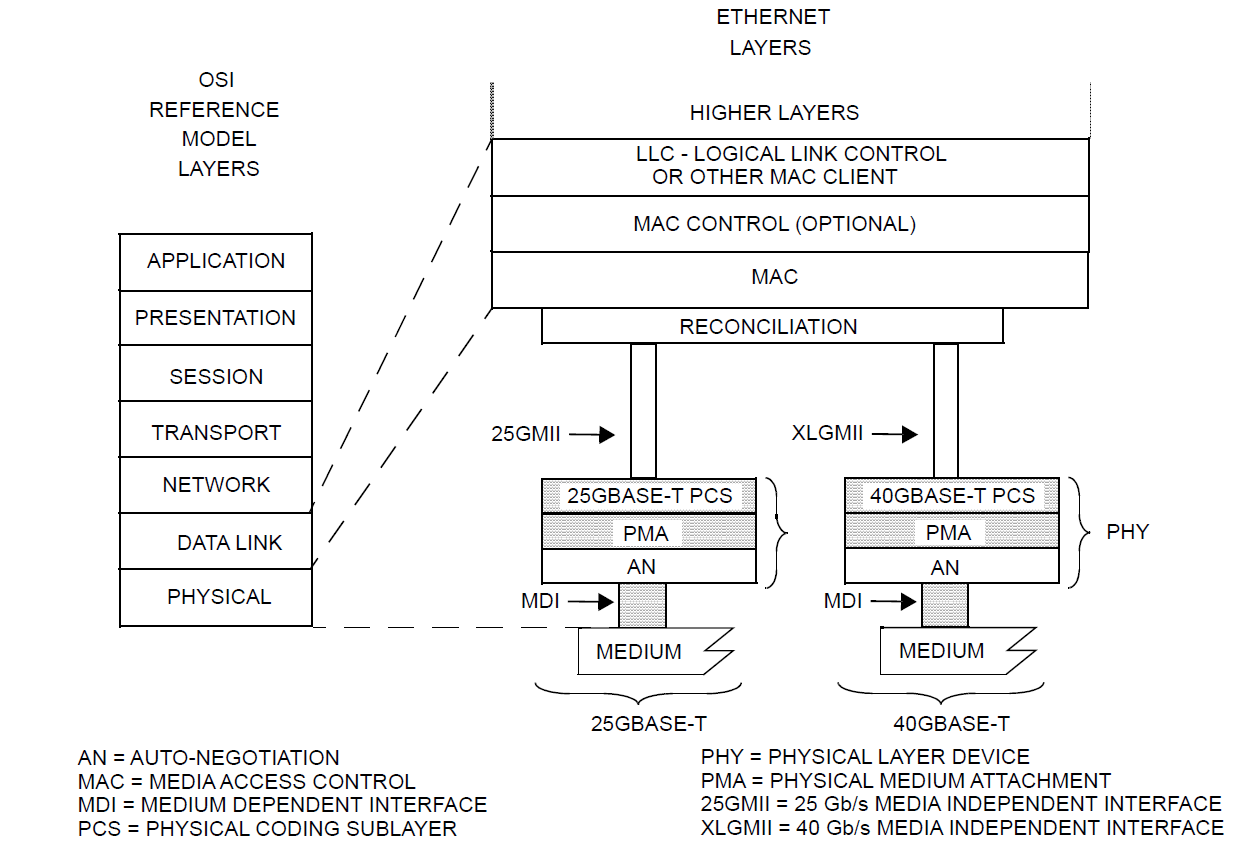
\includegraphics[width=\textwidth]{25-40-gbase-osi.png}
    \caption{Położenie 40GBASE-T w modelu OSI}
    \label{fig:40gbase-t_osi}
\end{figure}

\subsection{Media-Independent Interface}
MII czyli Media-Independent Interface to interfejs pomiędzy warstwą MAC oraz PHY. Powstał po to aby warstwy MAC oraz PHY były niezależne od siebie - pozwala na pracę kontrolera MAC z warstwą PHY, bez względu na to jakie medium jest w użyciu.
W technologii 40GBASE-T MII określany jest jako XLGMII. Składa się z dwóch wektorów 64-bitowych TXD i RXD - odpowiedzialne za przesył danych w obu kierunkach, dwóch wektorów 8-bitowych TXC i RXC - wykorzystywane do przesyłu sygnałów kontrolnych oraz TX\_CLK i RX\_CLK - którymi podawany jest sygnał zegara. XLGMII pozwala na przesył danych na poziomie 40 Gb/s, w obu kierunkach.

\subsection{Warstwa PCS}\label{subsection:pcs}
40GBASE-T PCS (Physical Coding Sublayer) jest warstwą odpowiedzialną m.in. za kodowanie i dekodowanie oraz skramblowanie i deskramblowanie. W jej skład wchodzą m.in. skrambler i deskrambler, kodery i dekodery RS-FEC i LDPC oraz układ mapujący bity na DSQ128.
Dane trafiają z warstwy MAC do PCS przez XLGMII i gromadzone są w 64-bitowe bloki. Po zebraniu 50 takich bloków, pierwsze 48 z nich transkodowane są w 512-bitowe bloki, a pozostałe są do nich dołączane. Dane są następnie skramblowane i dołączany jest do nich bit pomocniczy (auxiliary bit), po czym dzielone są na dwa zbiory --- pierwszy z nich trafia do kodera Reed-Solomona, a drugi przetwarzany jest przez koder LDPC (Low density parity check). Otrzymuje się w ten sposób $512*3$ bitów zakodowanych przez RS-FEC oraz $512*4$ bitów --- LDPC, które łączone są w 7-bitowe grupy  ($u_0$, $u_1$, $u_2$), ($c_0$, $c_1$, $c_2$, $c_3$).

\subsection{Modulacja w 40GBASE-T}
Technologia 40GBASE-T wykorzystuje 16-poziomową modulację PAM - mając 16 różnych poziomów amplitudy możemy zakodować 16 różnych wartości co daje nam 4 bity danych.
Oprócz bitów niosących dane, przesyła się również bity pomocnicze (auxiliary bits), przez co w rzeczywistości jeden symbol PAM16 koduje 3,125 bitów informacji.
W ciągu każdej sekundy przesyłanych jest 3200 milionów symboli co przekłada się na prędkość transmisji równą 10 Gb/s (3,125 bit/symbol * 3200 MBd) na każdej z czterech par skrętki, co sumarycznie daje transmisję 40 Gb/s.

\subsubsection{Double Square Quadrature Amplitude Modulation}
Jak opisano w \ref{subsection:pcs}, warstwa PCS koduje otrzymane dane w 7-bitowe grupy. W technologii 40GBASE-T symbole nadawane przez warstwę PMA wybierane są z konstelacji DSQ128 (Double Square Quadrature Amplitude Modulation).

Aby wyjaśnić czym jest DSQ128, pierw spójrzmy na modulację 64QAM. 64QAM (Quadrature Amplitude Modulation) to modulacja, która jest połączeniem modulacji amplitudy oraz fazy. Bity zamieniane są na symbole według diagramu konstelacji:

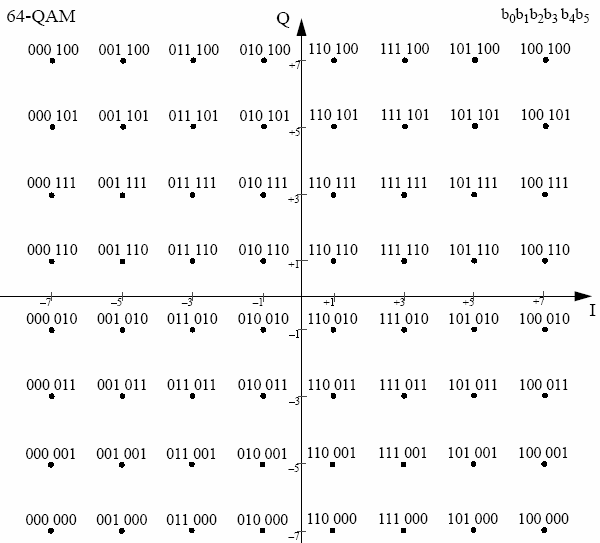
\includegraphics[scale=0.6]{64QAM-constellation-diagram.png}

Diagam podzielony jest na 4 sekcje, każda z nich zawiera 16 maksymalnie oddzielonych od siebie punktów. Punkty znajdujące się obok siebie różnią się jednym bitem --- dzięki czemu, gdy odbiorca otrzyma zły symbol, najprawdopodobniej tylko jeden bit będzie przekłamany.

DSQ128 jest złożeniem dwóch modulacji 64QAM i składa się z ośmiu sekcji, a każda z nich zawiera 16 punktów. Mając 7-bitową grupe ($u_0$, $u_1$, $u_2$), ($c_0$, $c_1$, $c_2$, $c_3$), pierwsze 3 bity definiują lewy dolny punkt w jednym z 8 regionów, natomiast na podstawie 4 kolejnych bitów wybierany jest jeden z 16 punktów w danym regionie. Proces ten opisany jest szczegółowo w \ref{mapowanie}

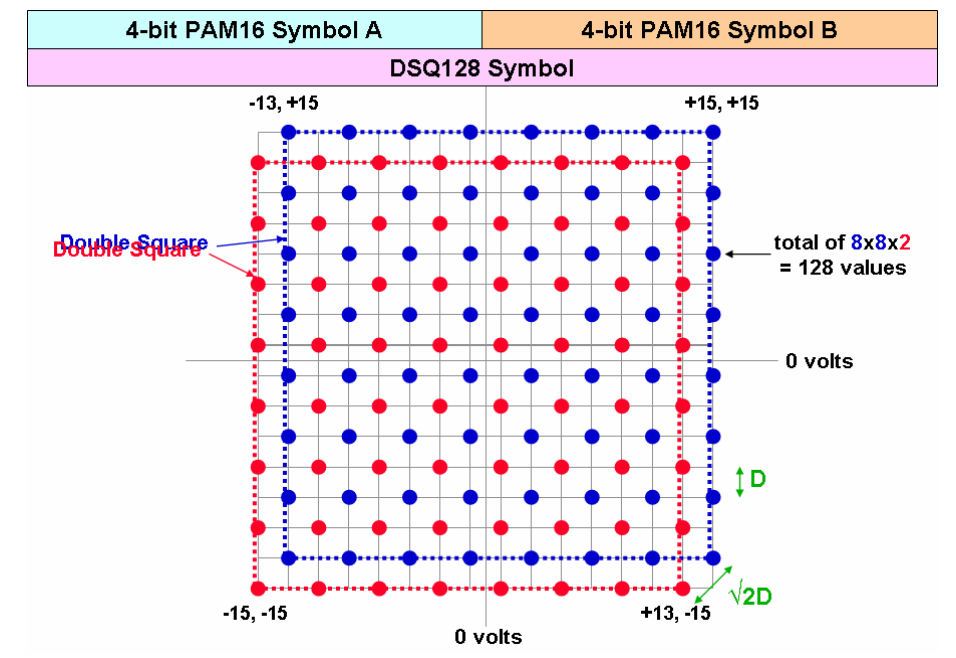
\includegraphics[scale=0.4]{dsq128.png}

\subsubsection{Mapowanie ramki LDPC na DSQ128}\label{mapowanie}
Zamianę 7-bitów ($u_0$, $u_1$, $u_2$), ($c_0$, $c_1$, $c_2$, $c_3$) pokazuje poniższy algorytm:

Krok 1:
\begin{align*}
    x_{13} &= \neg u_0 * u_2 \\
    x_{12} &= u_0 \oplus u_2 \\
    x_{11} &= c_0 \\
    x_{10} &= c_0 \oplus c_1 \\
    x_{23} &= (u_1 * u_2) + (u_0 * \neg u_1) \\
    x_{22} &= u_1 \oplus u_2 \\
    x_{21} &= c_2 \\
    x_{20} &= c_2 \oplus c_3
\end{align*}

Krok 2:
\begin{align*}
    x_1 &= 8x_{13} + 4x_{12} + 2x_{11} + x_{10} \\
    x_2 &= 8x_{23} + 4x_{22} + 2x_{21} + x_{20}
\end{align*}

Krok 3:
\begin{align*}
    y_1 &= (x_1 + x_2) \mod 16 \\
    y_2 &= (-x_1 + x_2) \mod 16
\end{align*}

Krok 4:
\begin{align*}
    \text{PAM16}_1 &= 2y_1 - 15 \\
    \text{PAM16}_2 &= 2y_2 - 15
\end{align*}

Otrzymane w ten sposób symbole są transmitowane na odpowiednich parach skrętki:

\begin{table}[h]
    \centering
    \resizebox{\textwidth}{!}{%
    \begin{tabular}{c | c c c c c c c |}
        \cmidrule{2-8}
        Pair A & PAM16$_1$<0> & PAM16$_2$<0> & PAM16$_1$<4> & PAM16$_2$<4> & \ldots & PAM16$_1$<508> & PAM16$_2$<508> \\
        \cmidrule{2-8}
        Pair B & PAM16$_1$<1> & PAM16$_2$<1> & PAM16$_1$<5> & PAM16$_2$<5> & \ldots & PAM16$_1$<509> & PAM16$_2$<509> \\
        \cmidrule{2-8}
        Pair C & PAM16$_1$<2> & PAM16$_2$<2> & PAM16$_1$<6> & PAM16$_2$<6> & \ldots & PAM16$_1$<510> & PAM16$_2$<510> \\
        \cmidrule{2-8}
        Pair D & PAM16$_1$<3> & PAM16$_2$<3> & PAM16$_1$<7> & PAM16$_2$<7> & \ldots & PAM16$_1$<511> & PAM16$_2$<511> \\
        \cmidrule{2-8}
    \end{tabular}}
\end{table}
